\documentclass{paper}
\usepackage{ctex}
\usepackage{geometry}
\geometry{a4paper, left=3.5cm, right=3.2cm, top=2.5cm, bottom=2.8cm}
\usepackage{orcidlink} % 用于 ORCID 链接
\usepackage{hyperref}
\hypersetup{colorlinks=true, linkcolor=black, urlcolor=blue}
\usepackage{amsmath} % 数学公式
\usepackage{amsfonts} % 数学字体
\usepackage{amssymb} % 数学符号
\usepackage{graphicx} % 插入图片
\usepackage{float} % 控制图片表格位置 [H]
\usepackage{caption} % 自定义标题
\usepackage{subcaption} % 子图
\usepackage{listings} % 代码
\usepackage{xcolor} % 颜色
\usepackage{enumitem} % 列表

% Custom color for code listings
\definecolor{codegreen}{rgb}{0,0.6,0}
\definecolor{codegray}{rgb}{0.5,0.5,0.5}
\definecolor{codepurple}{rgb}{0.58,0,0.82}
\definecolor{backcolour}{rgb}{0.95,0.95,0.92}

% Code listing style
\lstdefinestyle{mystyle}{
    backgroundcolor=\color{backcolour},   
    commentstyle=\color{codegreen},
    keywordstyle=\color{magenta},
    numberstyle=\tiny\color{codegray},
    stringstyle=\color{codepurple},
    basicstyle=\ttfamily\footnotesize,
    breakatwhitespace=false,         
    breaklines=true,                 
    captionpos=b,                    
    keepspaces=true,                 
    numbers=left,                    
    numbersep=5pt,                  
    showspaces=false,                
    showstringspaces=false,
    showtabs=false,                  
    tabsize=2
}
\lstset{style=mystyle}

\begin{document}

\title{基于时间序列和聚类的群聊行为分析}
\author{\href{https://github.com/F1Justin}{F1Justin} \and\href{https://github.com/Nameless-1313}{Nameless-1313} \and \href{https://github.com/duckgod782}{duckgod782}}
\date{\today}

\maketitle

\begin{abstract}
    本研究基于对7个高校东方Project爱好者QQ群的50余万条聊天记录进行分析,运用时间序列分析、K-means聚类和 LSTM 等方法,探究了用户行为模式及群体互动特征。研究发现群聊活动呈现明显的时间周期性,用户活跃度呈长尾分布;通过聚类分析识别出三类典型用户群体,揭示了不同活跃度用户的行为特征。研究结果为在线兴趣社群的用户行为理解与社群运营优化提供了数据支持和实证参考。
\end{abstract}

\setcounter{tocdepth}{2}
\tableofcontents

\section{引言}
\subsection{研究背景}
东方Project是一系列由上海爱丽丝幻乐团创作的同人作品,以其独特的弹幕射击游戏形式和丰富的幻想世界观而闻名,吸引了全球范围内的大量粉丝。其相关社群活跃于多种线上平台,其中QQ群作为中文社群的重要交流媒介,承载了丰富的用户行为与互动数据。

对QQ群聊数据的分析不仅能够揭示社群中用户行为的模式与特点,还能为社群管理、内容推荐以及用户体验优化提供数据支持。这种分析在理解社群动态与挖掘群体行为规律方面具有重要意义,同时为探索数字文化社群的研究提供了新的视角。

\subsection{研究问题}
本研究聚焦于基于东方Project相关QQ群的聊天记录,探索用户行为模式及群体活动规律。具体希望解答以下问题:

\begin{itemize}
    \item 用户在不同时段(如早晨、下午、晚上、深夜)的活跃模式是什么?这种模式是否因用户群体而异?
    \item 群聊活动是否存在周期性变化,例如日周期、周周期或更长时间尺度上的规律性?
    \item 用户之间的行为模式是否可以通过聚类分析进行分类,若可以,是否能够识别出特定的活跃用户群体及其行为特征?
    \item 如何利用时间序列分析方法预测未来群聊的活动趋势,为社群管理提供数据支持?
    \item 用户贡献在消息总量中的分布情况如何?是否存在少数用户主导群体活动的现象?
    \item 不同用户群体的文本特征(如常用关键词)如何影响其活跃行为及群体归属?
\end{itemize}

\section{数据描述}

本研究的数据来源于QQ群聊记录,采用自主搭建的 Nonebot2 机器人进行数据收集,主要使用以下插件实现数据存储与管理:

\begin{itemize}
    \item \textbf{nonebot-plugin-datastore} — 用于本地化储存。
    \item \textbf{nonebot-plugin-userinfo} — 获取用户信息。
    \item \textbf{nonebot-plugin-chatrecorder} — 实现消息存储,记录至 PostgreSQL 数据库。
\end{itemize}

在数据收集过程中,我们对参与者进行了充分的隐私保护,发布了《数据收集报告和隐私说明》,明确告知数据收集的范围、目的、使用方式及参与者的权利。以下是数据的具体描述:

\subsection{数据来源与收集方法}
本次数据收集涵盖了 7 个有效的QQ群,数据记录从 2024 年 8 月 27 日开始,至 12 月 24 日晚结束,总计约 50 万条聊天记录。数据通过 Nonebot 机器人自动记录,包括以下字段:
\begin{itemize}
    \item 消息内容:包含文本形式的消息。
    \item 时间戳:记录消息发送的具体时间。
    \item 群成员的公开昵称和 ID:不涉及真实姓名或其他敏感信息。
    \item 消息类型:包括普通文本消息和原始消息数据。
\end{itemize}

\subsection{数据预处理步骤}
为确保数据分析的准确性,数据预处理包括以下步骤:
\begin{itemize}
    \item \textbf{机器人用户过滤}:排除由机器人生成的消息,确保数据代表真实用户的行为。
    \item \textbf{时间转换}:将所有时间戳统一转换为东八区时间,便于时段分析。
    \item \textbf{分组存储与优化}:根据群号对数据分组存储,并使用多线程优化数据加载速度。
\end{itemize}

这些数据为后续的时间序列分析和话题挖掘提供了坚实基础,有助于揭示群体行为模式及其演变规律。

\section{数据探索性分析}

\subsection{数据概览}

在本次研究的数据集中,经过预处理后,包含以下核心统计信息:

\begin{itemize}
    \item \textbf{总消息数}: 数据集中共有 501,636 条有效聊天记录。
    \item \textbf{总用户数}: 记录到的独立用户数为 772 名。
    \item \textbf{总群组数}: 涉及的群组总计 7 个。
\end{itemize}

为进一步了解各群组在整体数据中的贡献比例,我们对每个群组的消息数量进行了统计,并绘制了消息分布图(对消息数采用对数刻度处理)。如图1 所示,不同群组的消息量存在显著差异,部分群组的消息数量显著高于其他群组。

\begin{figure}[H]
    \centering
    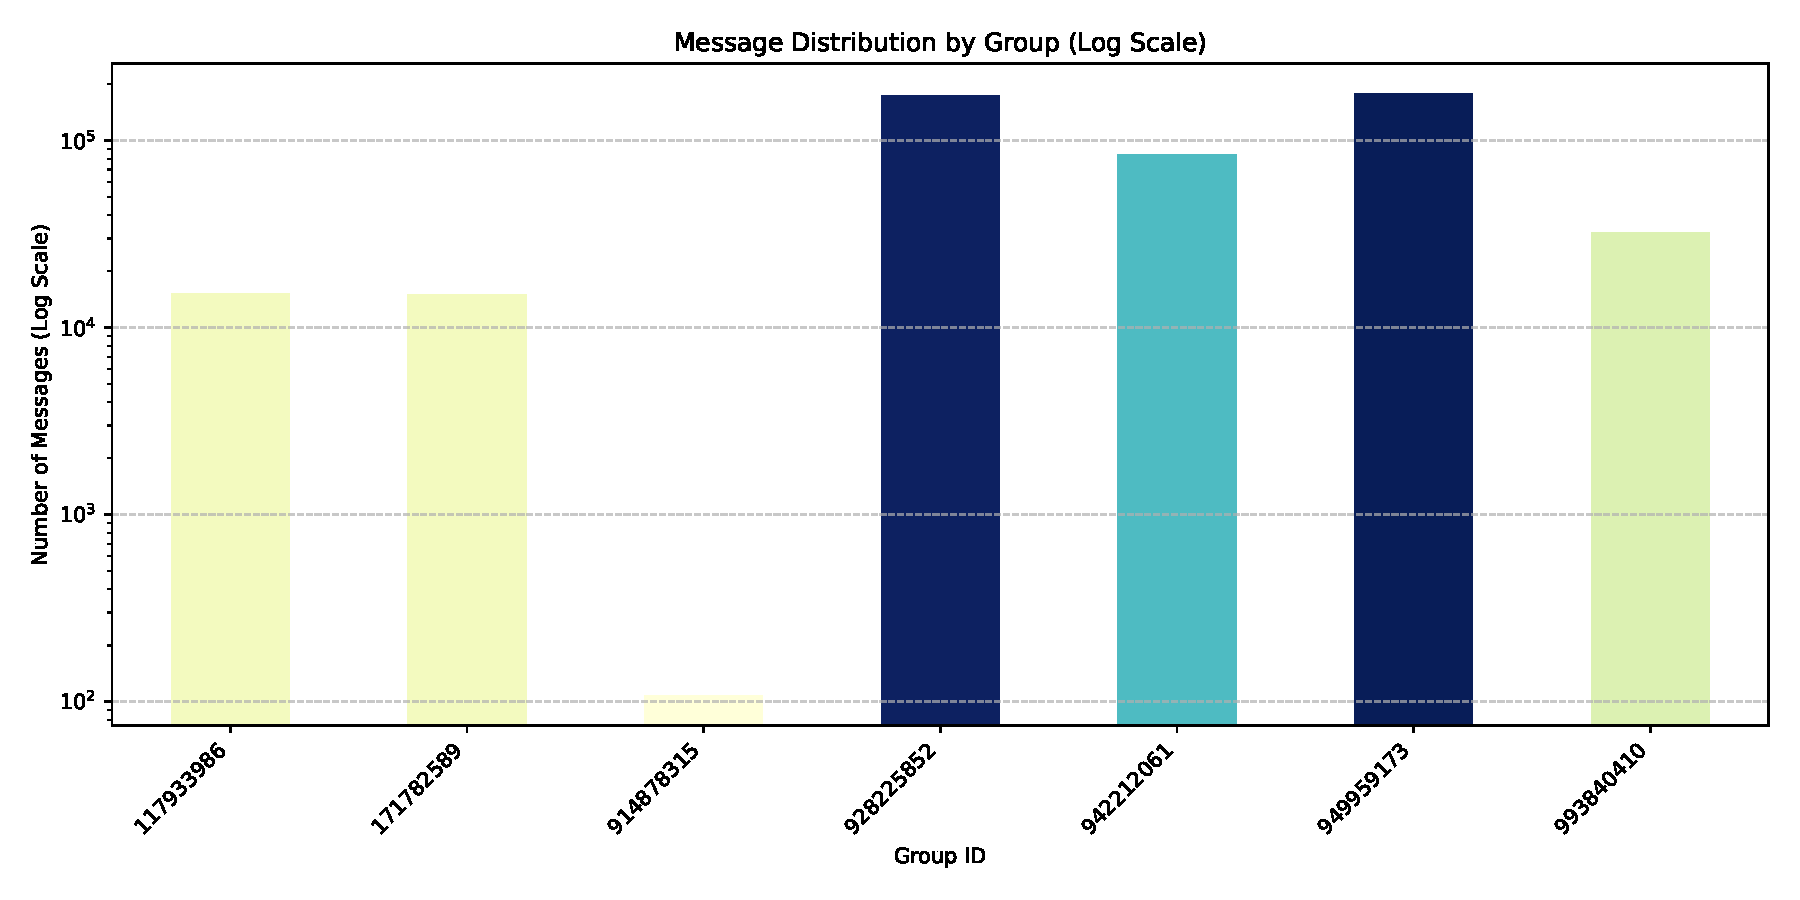
\includegraphics[width=0.9\textwidth]{/Users/justin/Desktop/data_analysis/graphs/MessageDistributionbyGroup(LogScale).pdf}
    \caption{各群组消息分布(对数刻度)}
    \label{fig:1}
\end{figure}

从图中可以看出,部分群组活跃度较高,其消息数量占据了总量的大部分,而其他群组的消息量相对较少。这一分布特征为后续的用户行为模式分析提供了重要背景依据。

\subsection{用户行为分析}

基于用户消息数据的统计分析结果如下:

\begin{itemize}
    \item \textbf{用户消息数量分布}: 
    本数据集包含 772 名用户,总消息数为 501,636 条。用户消息数量分布的描述性统计如下:
    \begin{itemize}
        \item 平均消息数: 639.82
        \item 中位数消息数: 36.00
        \item 最大消息数: 21,091
        \item 最小消息数: 1
        \item 标准差: 1,870.98
        \item 25\% 分位数: 5.00
        \item 75\% 分位数: 300.50
    \end{itemize}
    此外,消息区间内用户数量分布如图2 所示(对用户数采用对数刻度处理),显示消息量集中于较少用户。

    \begin{figure}[H]
        \centering
        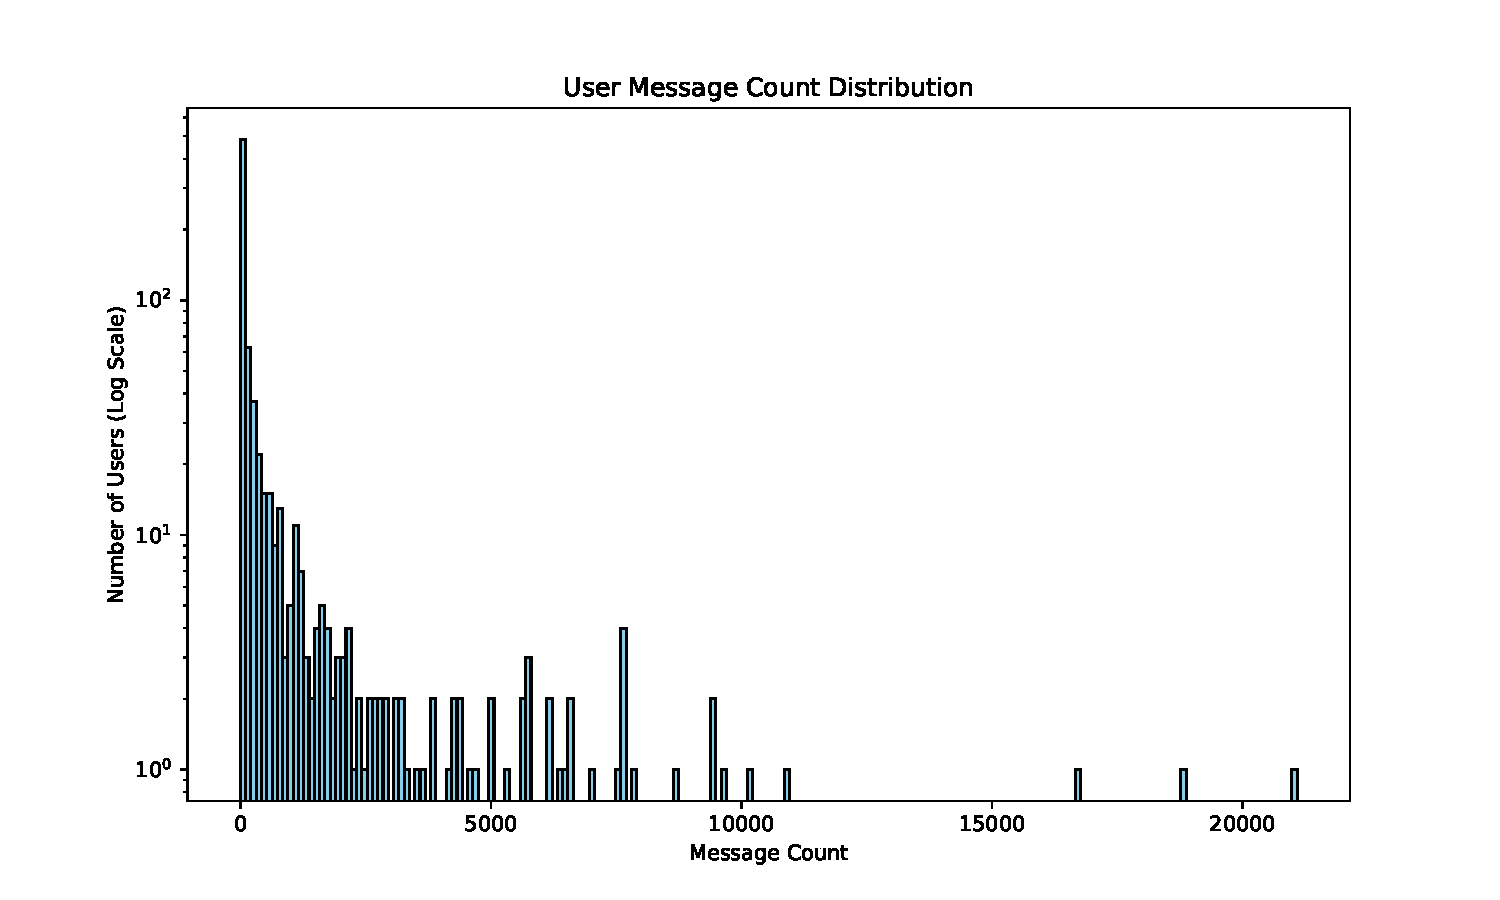
\includegraphics[width=0.8\textwidth]{/Users/justin/Desktop/data_analysis/graphs/NumberofUsers(LogScale).pdf}
        \caption{用户消息数量分布(对数刻度)}
        \label{fig:2}
    \end{figure}

    \item \textbf{相对活跃用户比例}: 
    发送超过 100 条消息的用户比例为 38.34\%。这一群体的用户对总消息量贡献较大。

    \item \textbf{用户活跃度分类}: 
    根据每位用户的消息数量,我们引入平均每用户发送消息数量 $c$ 的倍数关系作为划分标准,将用户分为以下四个活跃度级别:
    \begin{enumerate}
        \item 不活跃用户(1-63 条消息):427 人,总计贡献了 5,408 条消息。
        \item 低活跃用户(64-639 条消息):209 人,总计贡献了 47,901 条消息。
        \item 活跃用户(640-6398 条消息):117 人,总计贡献了 252,976 条消息。
        \item 水群领域大神(大于 6398 条消息):19 人,总计贡献了 187,658 条消息。
    \end{enumerate}
    活跃用户和水群领域大神的消息贡献比例尤为显著。

\end{itemize}

\begin{figure}[H]
    \centering
    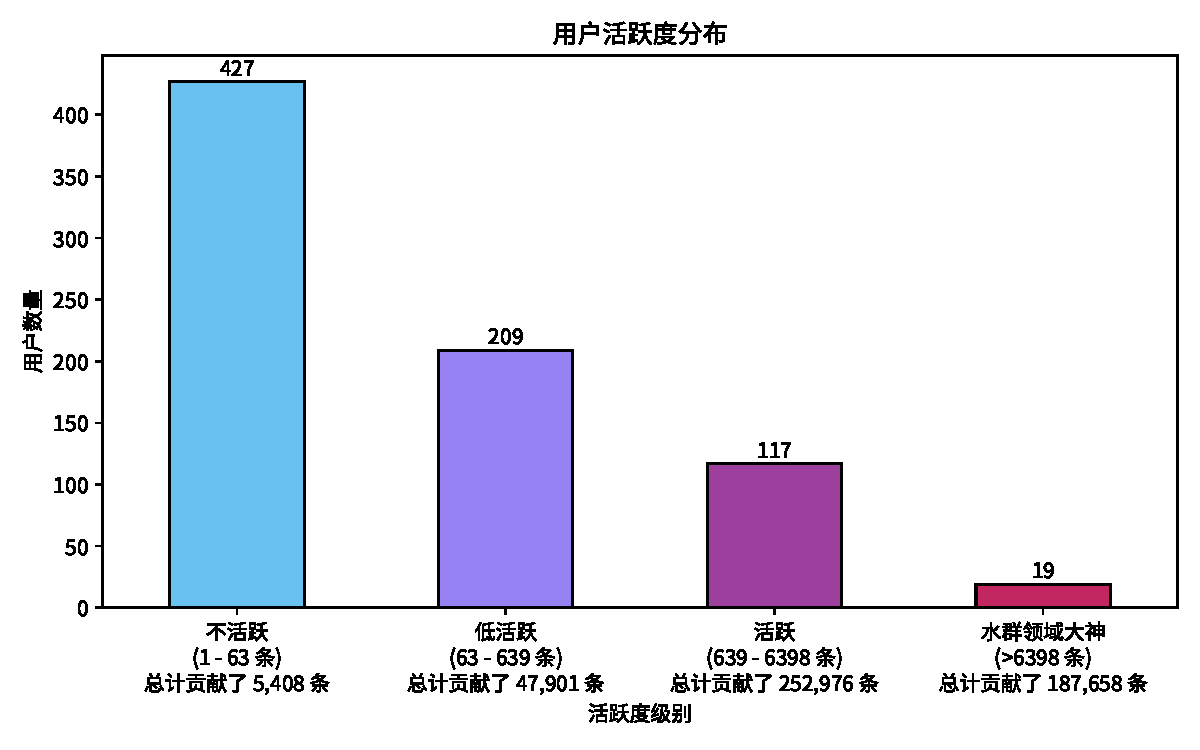
\includegraphics[width=0.8\textwidth]{/Users/justin/Desktop/data_analysis/graphs/activity_levels.pdf}
    \caption{用户活跃度分类}
    \label{fig:3}
\end{figure}

\subsection{时间维度分析}

消息数据在时间维度上的分布呈现以下特点:

\begin{itemize}
    \item \textbf{小时消息分布}: 
    消息量在一天内呈现周期性变化,高峰时段为 10:00 至次日 1:00。每小时的消息量如图4 所示,白天自 6 点逐步升高,在 11 点达到区间极大值并开始回落;自 15 时开始又逐渐升高至18时达到区间极大值并回落;自21 点再次开始升高,凌晨 1 点达到最大值。

    \item \textbf{周消息分布}:
    按星期统计,工作日(周一至周五)的消息量较高,而周末(周六和周日)消息量有所下降。具体分布如图5 (a) 所示。

    \item \textbf{周消息量变化}:
    消息量按周统计如图5 (b) 所示,显示消息量在最近几周内总体呈增长趋势。
\end{itemize}

\begin{figure}[H]
    \centering
    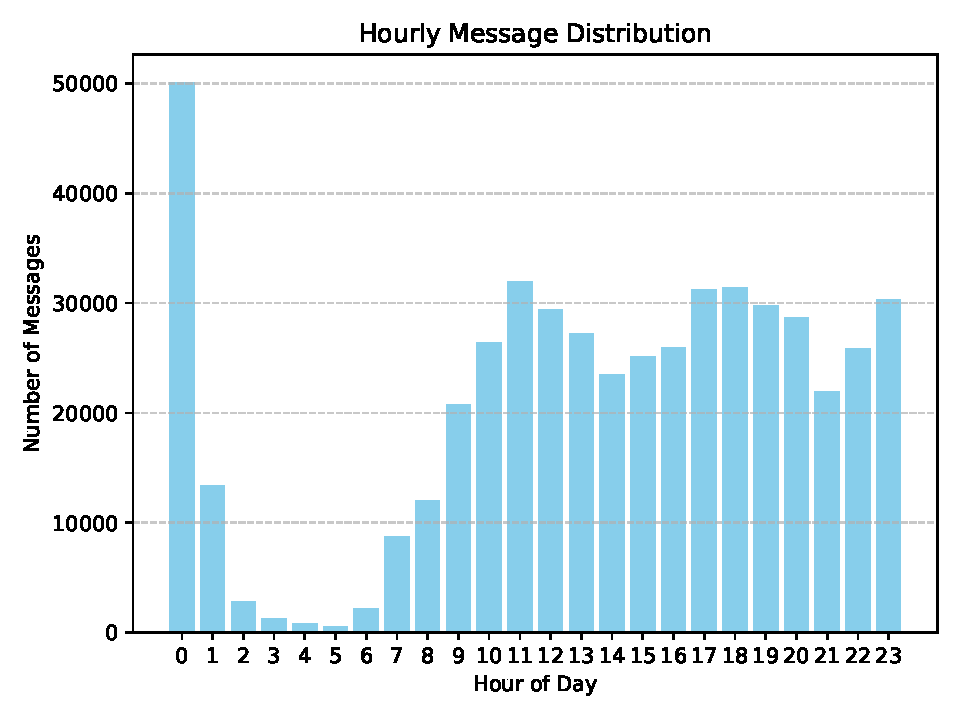
\includegraphics[width=0.75\textwidth]{/Users/justin/Desktop/data_analysis/graphs/HourlyMessageDistribution.pdf}
    \caption{每小时消息分布}
    \label{fig:hourly_msg_dist}
\end{figure}
\begin{figure}[H]
    \centering
    \begin{subfigure}[b]{0.45\textwidth}
        \centering
        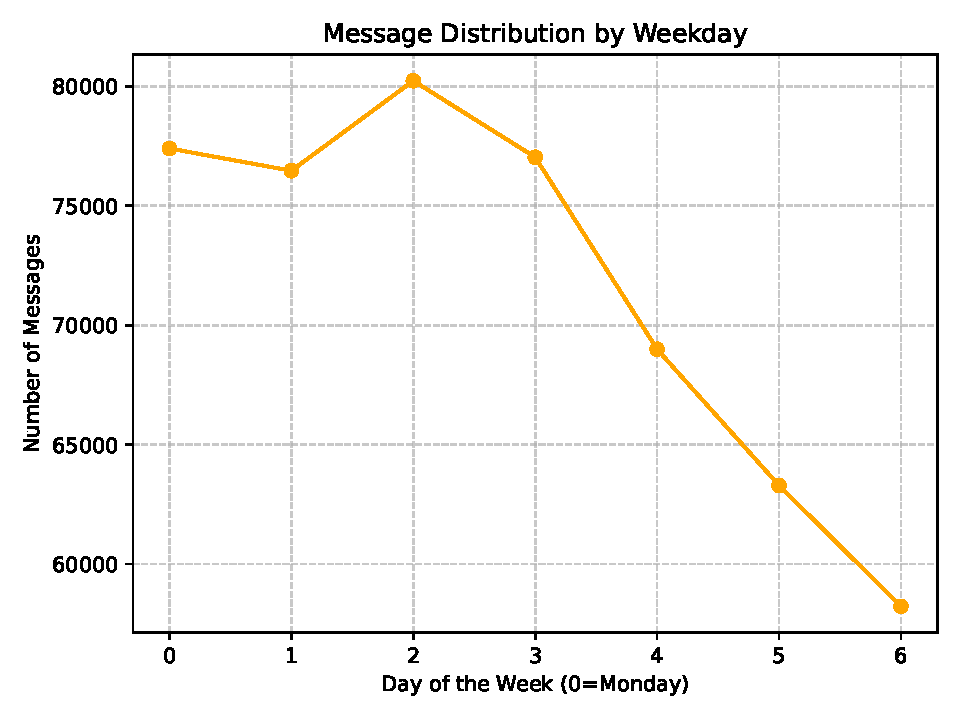
\includegraphics[width=\textwidth]{/Users/justin/Desktop/data_analysis/graphs/MessageDistributionbyWeekday.pdf}
        \caption{按星期统计的消息量分布}
        \label{fig:weekday_msg_dist}
    \end{subfigure}
    \hfill
    \begin{subfigure}[b]{0.45\textwidth}
        \centering
        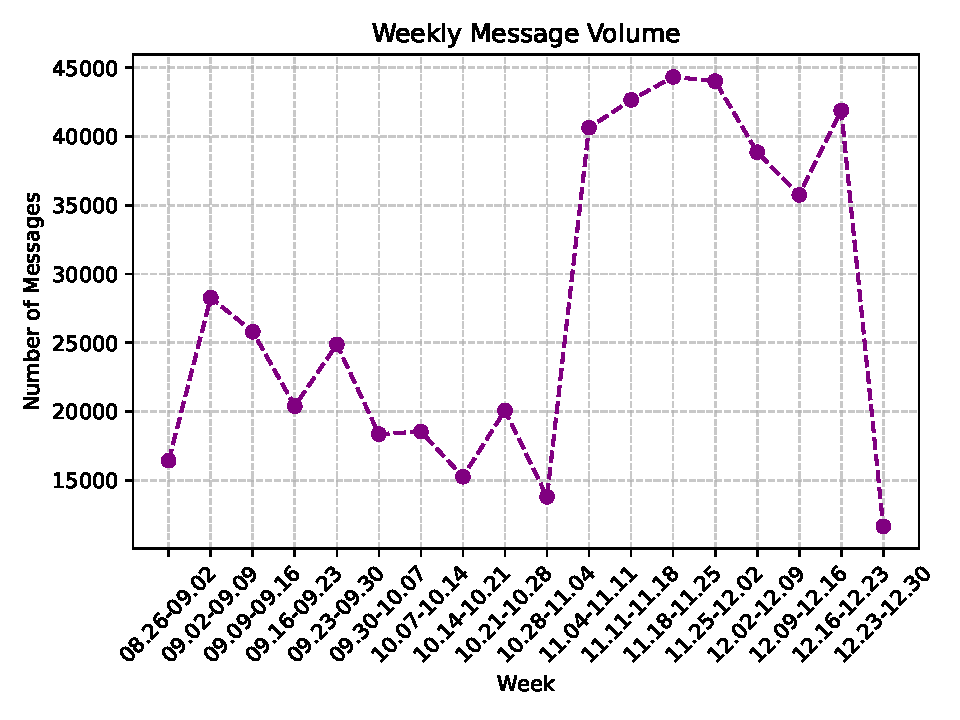
\includegraphics[width=\textwidth]{/Users/justin/Desktop/data_analysis/graphs/WeeklyMessageVolume.pdf}
        \caption{按周统计的消息量变化}
        \label{fig:weekly_msg_vol}
    \end{subfigure}
    \caption{消息量分布}
    \label{fig:msg_dist}
\end{figure}

\subsection{内容分析}
\begin{figure}[H]
    \centering
    
\includegraphics[width=0.7\textwidth]{/Users/justin/Desktop/data_analysis/graphs/WordCloud.png}
    \caption{高频词汇词云}
    \label{fig:wordcloud}
\end{figure}
\begin{itemize}
\item 高频词汇与主题词\\
图 6 为消息最多的群聊生成的词云,展示了聊天中高频出现的词汇。主要主题包括常用日常词汇、群聊热点话题,以及特定兴趣领域相关的关键词(如“fumo”、“莉莉”、“东方”等),反映了群组的兴趣及互动内容。

\item 消息类型统计(文本、图片、表情等)\\ 
图 7 为全部群聊消息类型的分布情况。结果显示:
\begin{itemize}
    \item 文本消息占比最高,为 71.6\%,是主要的交流方式。
    \item 图片消息占 13.8\%,显示了成员通过图片进行互动的频率。
    \item 表情消息占 6.2\%,说明了表情在丰富聊天氛围中的重要作用。
    \item 卡片消息(JSON格式)占 8.4\%,反映了转发消息或机器人功能的使用情况。
\end{itemize}

\end{itemize}

\begin{figure}[H]
    \centering
    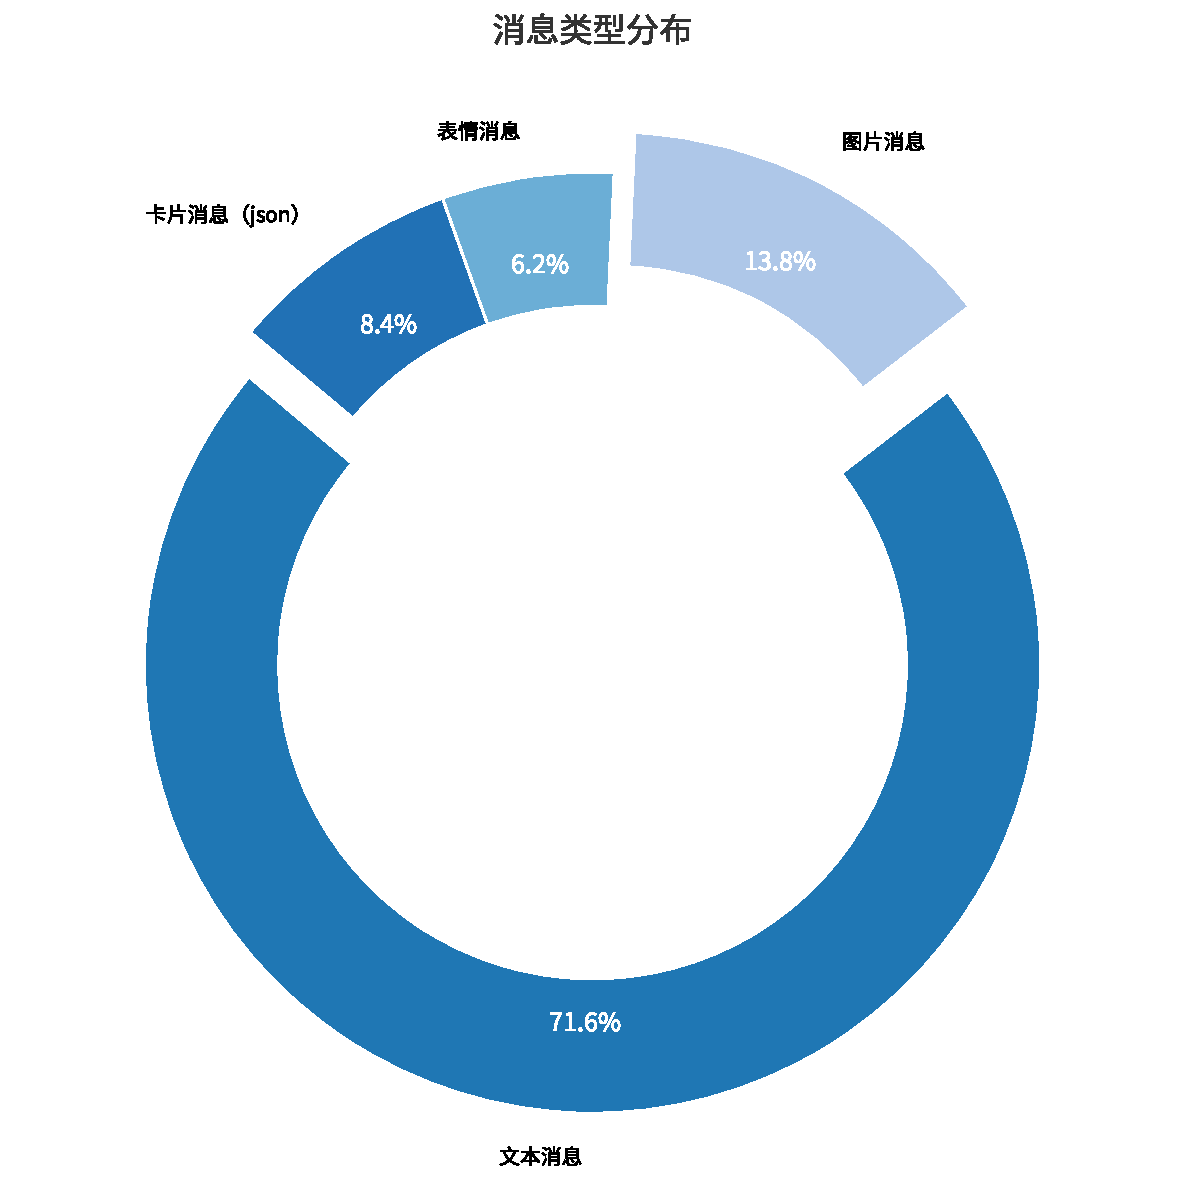
\includegraphics[width=0.55\textwidth]{/Users/justin/Desktop/data_analysis/graphs/MessageTypeDistribution.pdf}
    \caption{消息类型分布}
    \label{fig:msg_type_dist}
\end{figure}

\section{聚类分析}

除了上述简单的统计外,本报告还采用了 K-Means 聚类算法对用户行为数据进行分析,并结合 PCA 和 t-SNE 两种降维技术进行可视化,旨在识别用户群体的不同行为模式。

\subsection{技术原理}
\subsubsection{K-Means 聚类}
K-Means 是一种无监督学习算法,其目标是将数据点划分为 $k$ 个簇,使得每个簇内的点之间距离最小,而不同簇之间的点相距较远。具体来说,K-Means 通过最小化以下目标函数来完成聚类:
\[
J = \sum_{i=1}^k \sum_{x \in C_i} \| x - \mu_i \|^2
\]
其中,$C_i$ 是第 $i$ 个簇的集合,$\mu_i$ 是第 $i$ 个簇的质心,$\| x - \mu_i \|^2$ 是数据点 $x$ 到质心 $\mu_i$ 的欧氏距离平方。

算法的主要步骤如下:
\begin{enumerate}
    \item 初始化:随机选择 $k$ 个点作为初始质心。
    \item 分配:将每个数据点分配到距离最近的质心所在的簇:
    \[
    C_i = \{x : \| x - \mu_i \|^2 \leq \| x - \mu_j \|^2, \, \forall j \neq i \}
    \]
    \item 更新:重新计算每个簇的质心为簇内点的均值:
    \[
    \mu_i = \frac{1}{|C_i|} \sum_{x \in C_i} x
    \]
    \item 迭代:重复执行分配和更新步骤,直至质心不再显著变化或达到最大迭代次数。
\end{enumerate}

\subsubsection{主成分分析 (PCA)}
主成分分析 (Principal Component Analysis, PCA) 是一种线性降维方法,其目标是通过寻找数据的主要变异方向,将高维数据投影到一个低维子空间。PCA 的核心是最大化投影后的方差,同时保持投影方向之间的正交性。

PCA 的目标函数为:
\[
\text{maximize } \| W^T X \|^2 \quad \text{subject to } W^T W = I
\]
其中,$X$ 是数据矩阵,$W$ 是降维的变换矩阵。通过计算数据的协方差矩阵并求解特征值和特征向量,选取前 $d$ 个特征向量作为降维方向。

\subsubsection{t-SNE}
t-SNE (t-Distributed Stochastic Neighbor Embedding) 是一种非线性降维技术,专注于保留数据的局部结构。t-SNE 的核心思想是:
\begin{itemize}
    \item 在高维空间中,将数据点之间的距离转化为条件概率分布:
    \[
    P_{j|i} = \frac{\exp(-\|x_i - x_j\|^2 / 2\sigma_i^2)}{\sum_{k \neq i} \exp(-\|x_i - x_k\|^2 / 2\sigma_i^2)}
    \]
    \item 在低维空间中构造相应的条件概率分布 $Q_{j|i}$,并最小化两个分布之间的 Kullback-Leibler (KL) 散度:
    \[
    KL(P||Q) = \sum_i \sum_j P_{j|i} \log \frac{P_{j|i}}{Q_{j|i}}
    \]
\end{itemize}

\subsection{技术过程}

\subsubsection{数据准备}
\begin{enumerate}
    \item 从指定目录中读取所有 CSV 文件并整合到一个 DataFrame 中。
    \item 填充缺失用户 ID,剔除机器人用户和无效用户 ID。
    \item 转换时间戳数据为时间类型,并计算用户在不同时间段的活跃度。
\end{enumerate}

\subsubsection{特征提取}
\begin{enumerate}
    \item 使用 TF-IDF 对用户文本数据进行向量化处理,提取前 10 个高频词作为文本特征。
    \item 对数值特征(如消息总数和各时间段消息数)进行标准化,确保不同量纲特征的均衡性。
\end{enumerate}

\subsubsection{聚类分析}
\begin{enumerate}
    \item 使用标准化的数值特征与文本特征向量,构建用户行为数据矩阵。
    \item 采用 K-Means 算法,将用户分为 3 个簇。
\end{enumerate}

\subsubsection{降维与可视化}
\begin{enumerate}
    \item 使用 PCA 对文本特征向量提取前两个主成分,并绘制聚类结果的二维散点图。
    \item 使用 t-SNE 对文本特征向量进一步展示用户在局部结构上的分布。
    \end{enumerate}

\subsection{结果分析}
聚类结果将用户分为以下三类:
\begin{itemize}
    \item Cluster 0: 中度活跃用户,总消息数平均为 3402.57,主要活跃在上午和下午。
    \item Cluster 1: 低活跃用户,规模最大,总消息数平均为 325.45,各时间段活跃度较低。
    \item Cluster 2: 高活跃用户,总消息数平均为 7068.80,上午、下午和夜间活跃度均较高。
\end{itemize}
从群体规模来看,用户活跃度呈现出明显的长尾分布特征,绝大多数用户属于低活跃度群体,而高度活跃用户仅占很小比例。

通过降维方法进行可视化,PCA结果展示了数据的主要变异方向,用户在第一主成分上的分布与其活跃度水平呈现良好的对应关系,这表明消息总量是区分用户群体的主要特征。虽然t-SNE在局部结构的展示上表现出更强的区分度,将低活跃度用户分散到多个相对独立的区域,但这种表现可能过分强调了低活跃用户群体内部的微小差异,反而模糊了群体间的本质区别。


\begin{figure}[H]
        \centering
        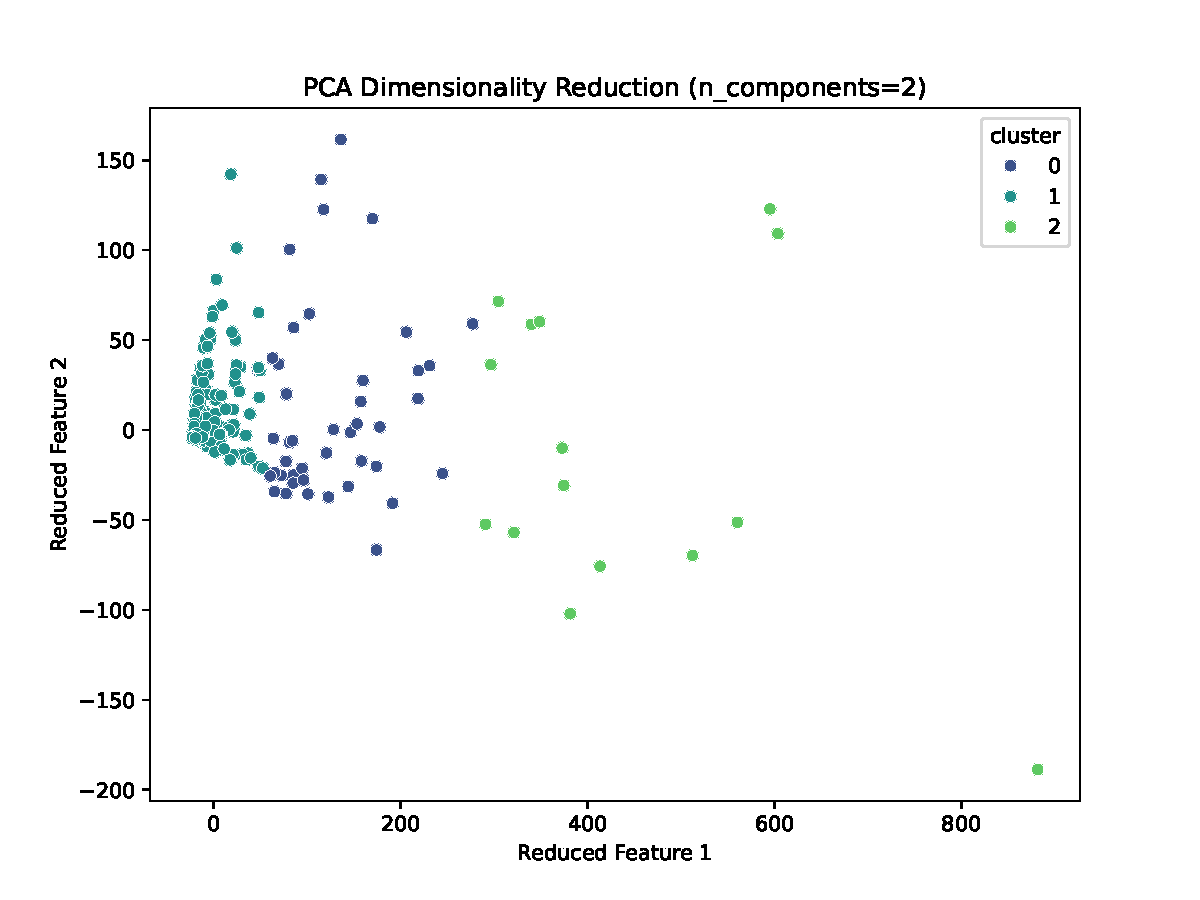
\includegraphics[width=0.8\textwidth]{/Users/justin/Desktop/data_analysis/graphs/output_pca.pdf}
        \caption{PCA 降维结果}
        \label{fig:pca}
\end{figure}
\begin{figure}[H]
        \centering
        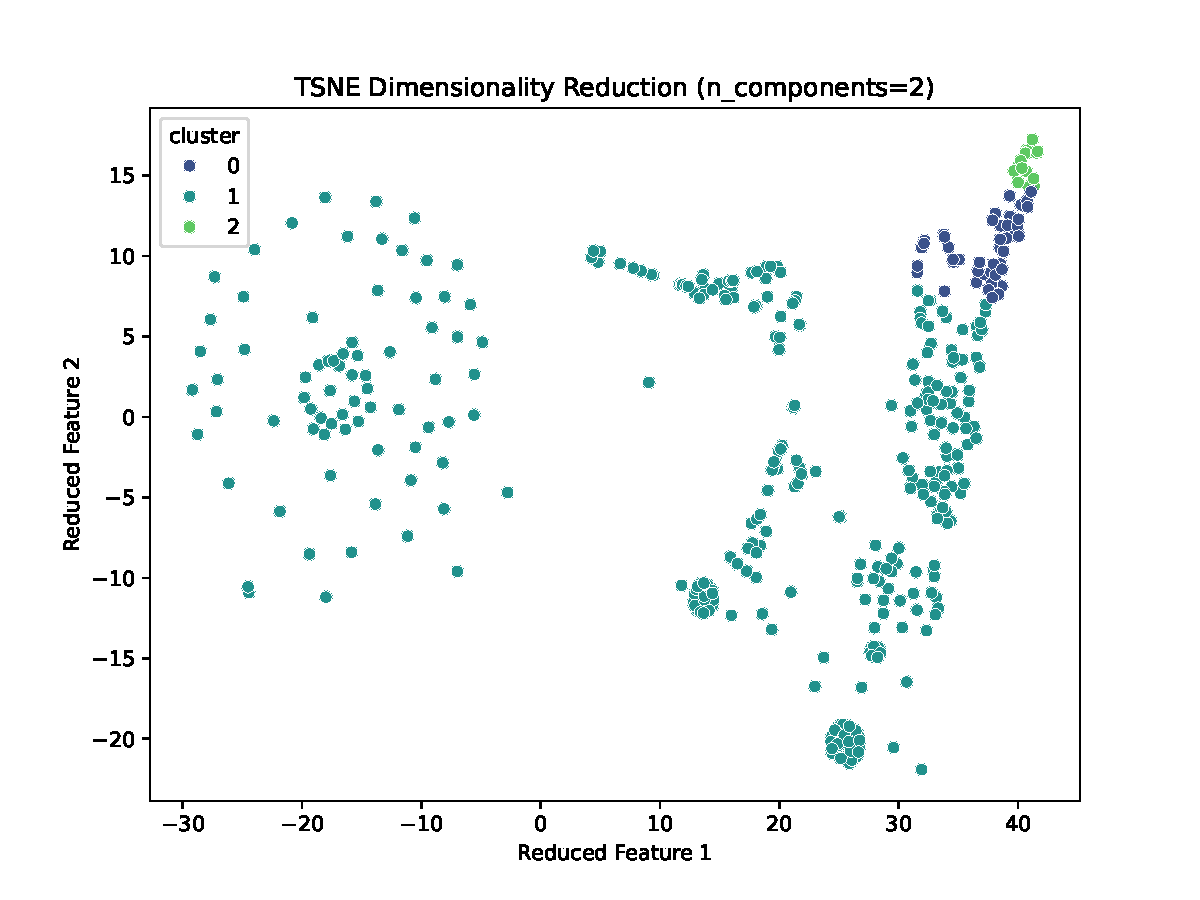
\includegraphics[width=0.8\textwidth]{/Users/justin/Desktop/data_analysis/graphs/output_tsne.pdf}
        \caption{t-SNE 降维结果}
        \label{fig:tsne}
\end{figure}

\section{LSTM 时间序列预测}

\subsection{技术原理}

本部分采用长短期记忆网络(Long Short-Term Memory, LSTM)对群聊各时段的消息数量进行时间序列预测。LSTM 是一种特殊的循环神经网络(Recurrent Neural Network, RNN),特别适合处理和预测时间序列数据,因为它能够捕获序列中的长期依赖关系。

LSTM 的核心组件是其 \textbf{单元结构},包括三个门控机制:输入门(Input Gate)、遗忘门(Forget Gate)和输出门(Output Gate)。这些门控机制通过选择性地记住或遗忘历史信息,解决了传统 RNN 中的梯度消失和梯度爆炸问题。

\begin{itemize}
    \item \textbf{遗忘门}:决定当前时刻哪些信息需要遗忘。
    \[
    f_t = \sigma(W_f \cdot [h_{t-1}, x_t] + b_f)
    \]
    其中,$f_t$ 是遗忘门的输出,$h_{t-1}$ 是上一时刻的隐藏状态,$x_t$ 是当前输入,$W_f$ 和 $b_f$ 是权重和偏置,$\sigma$ 是 sigmoid 激活函数。

    \item \textbf{输入门}:决定当前时刻哪些信息需要更新。
    \[
    i_t = \sigma(W_i \cdot [h_{t-1}, x_t] + b_i)
    \]
    \[
    \tilde{C}_t = \tanh(W_c \cdot [h_{t-1}, x_t] + b_c)
    \]
    其中,$i_t$ 是输入门的输出,$\tilde{C}_t$ 是候选记忆状态。

    \item \textbf{记忆更新}:将遗忘门和输入门的输出结合,更新记忆单元。
    \[
    C_t = f_t \odot C_{t-1} + i_t \odot \tilde{C}_t
    \]
    其中,$\odot$ 表示元素逐项相乘。

    \item \textbf{输出门}:决定当前时刻的输出状态。
    \[
    o_t = \sigma(W_o \cdot [h_{t-1}, x_t] + b_o)
    \]
    \[
    h_t = o_t \odot \tanh(C_t)
    \]
    其中,$o_t$ 是输出门的输出,$h_t$ 是当前时刻的隐藏状态,也是 LSTM 的最终输出。
\end{itemize}

\subsection{应用于时间序列预测}

在本次分析中,我们将各时段的消息数量视为时间序列数据,使用 LSTM(Long Short-Term Memory)模型来学习其动态变化规律,并预测未来某一时段的消息数量。以下是具体的研究步骤、结果和改进建议。

\subsection*{1. 数据准备}
\begin{enumerate}[label=(\alph*)]
    \item \textbf{数据分割}:将时间序列数据分割为固定长度的输入序列 $X$ 和对应的目标值 $y$。输入序列长度由参数 $seq\_length$ 决定。
    \item \textbf{归一化处理}:使用 \texttt{MinMaxScaler} 将数据标准化至 $[0, 1]$ 区间,公式如下:
    \[
    x' = \frac{x - \min(x)}{\max(x) - \min(x)}
    \]
    此步骤旨在加快模型的训练速度并提高预测精度。
\end{enumerate}

\subsection*{2. 模型训练}
\begin{enumerate}[label=(\alph*)]
    \item \textbf{网络构建}:搭建 LSTM 模型架构,包括以下部分:
    \begin{itemize}
        \item 单层或多层 LSTM 层,用于捕获时间序列的短期和长期依赖关系。
        \item 全连接层(Dense Layer),将 LSTM 层的输出映射为预测值。
    \end{itemize}
    \item \textbf{损失函数}:使用均方误差(Mean Squared Error, MSE)作为优化目标:
    \[
    \text{MSE} = \frac{1}{n} \sum_{i=1}^n (\hat{y}_i - y_i)^2
    \]
    其中,$\hat{y}_i$ 是预测值,$y_i$ 是实际值,$n$ 是样本数。
    \item \textbf{优化方法}:采用 Adam 优化器,通过反向传播算法(Backpropagation Through Time, BPTT)更新模型权重。
\end{enumerate}



\subsection*{3. 预测和评估}
\begin{enumerate}[label=(\alph*)]
    \item \textbf{预测过程}:使用训练好的 LSTM 模型对测试集数据进行预测,并反向缩放至原始数据范围。
    \item \textbf{性能评估}:使用以下指标评估模型性能:
    \begin{itemize}
        \item \textbf{均方误差(MSE)}:
        \[
        \text{MSE} = \frac{1}{n} \sum_{i=1}^n (\hat{y}_i - y_i)^2
        \]
        \item \textbf{均方根误差(RMSE)}:
        \[
        \text{RMSE} = \sqrt{\text{MSE}}
        \]
        \item \textbf{平均绝对误差(MAE)}:
        \[
        \text{MAE} = \frac{1}{n} \sum_{i=1}^n \lvert \hat{y}_i - y_i \rvert
        \]
    \end{itemize}
    \item \textbf{结果分析}:测试集上的误差指标如下:
    \begin{itemize}
        \item 均方误差(MSE):2447.03, 4007.12
        \item 均方根误差(RMSE):49.47, 63.30
        \item 平均绝对误差(MAE):34.88, 44.69
    \end{itemize}
    这些结果表明模型对大部分数据的预测较为准确,但仍存在一定程度的误差。
\end{enumerate}

\begin{figure}[H]
    \centering
    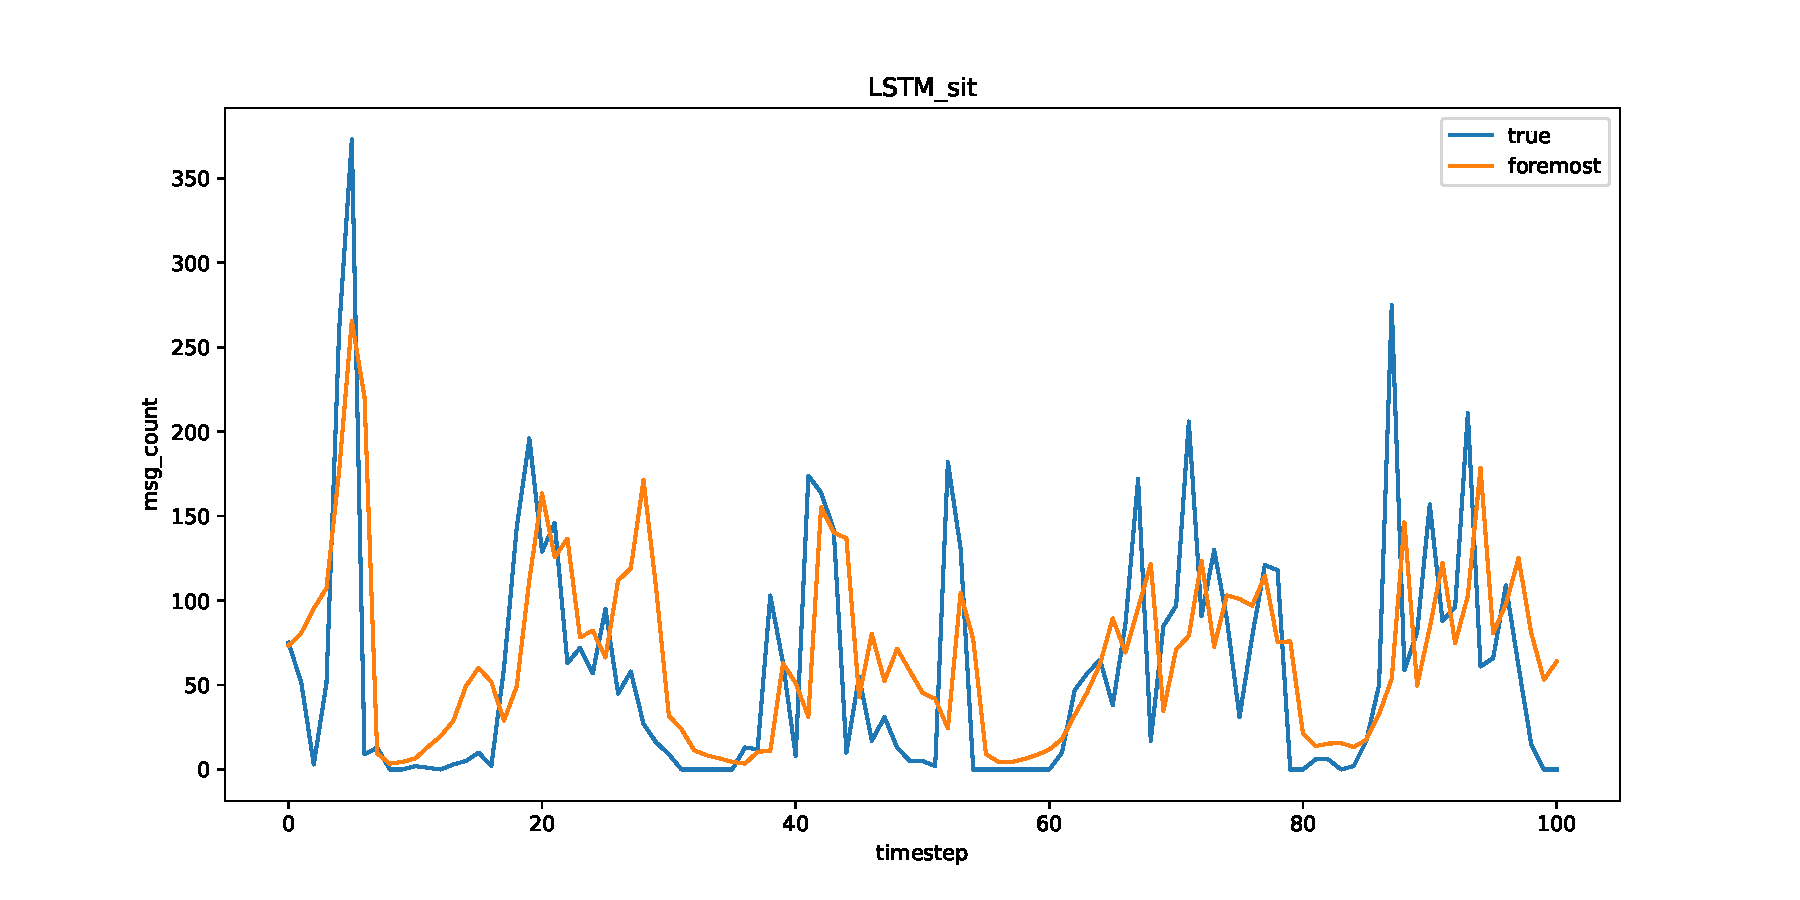
\includegraphics[width=0.8\textwidth]{/Users/justin/Desktop/data_analysis/graphs/LSTM_sit.pdf}
    \caption{LSTM 时间序列预测结果(sit)}
    \label{fig:lstm_sit}
\end{figure}

\begin{figure}[H]
    \centering
    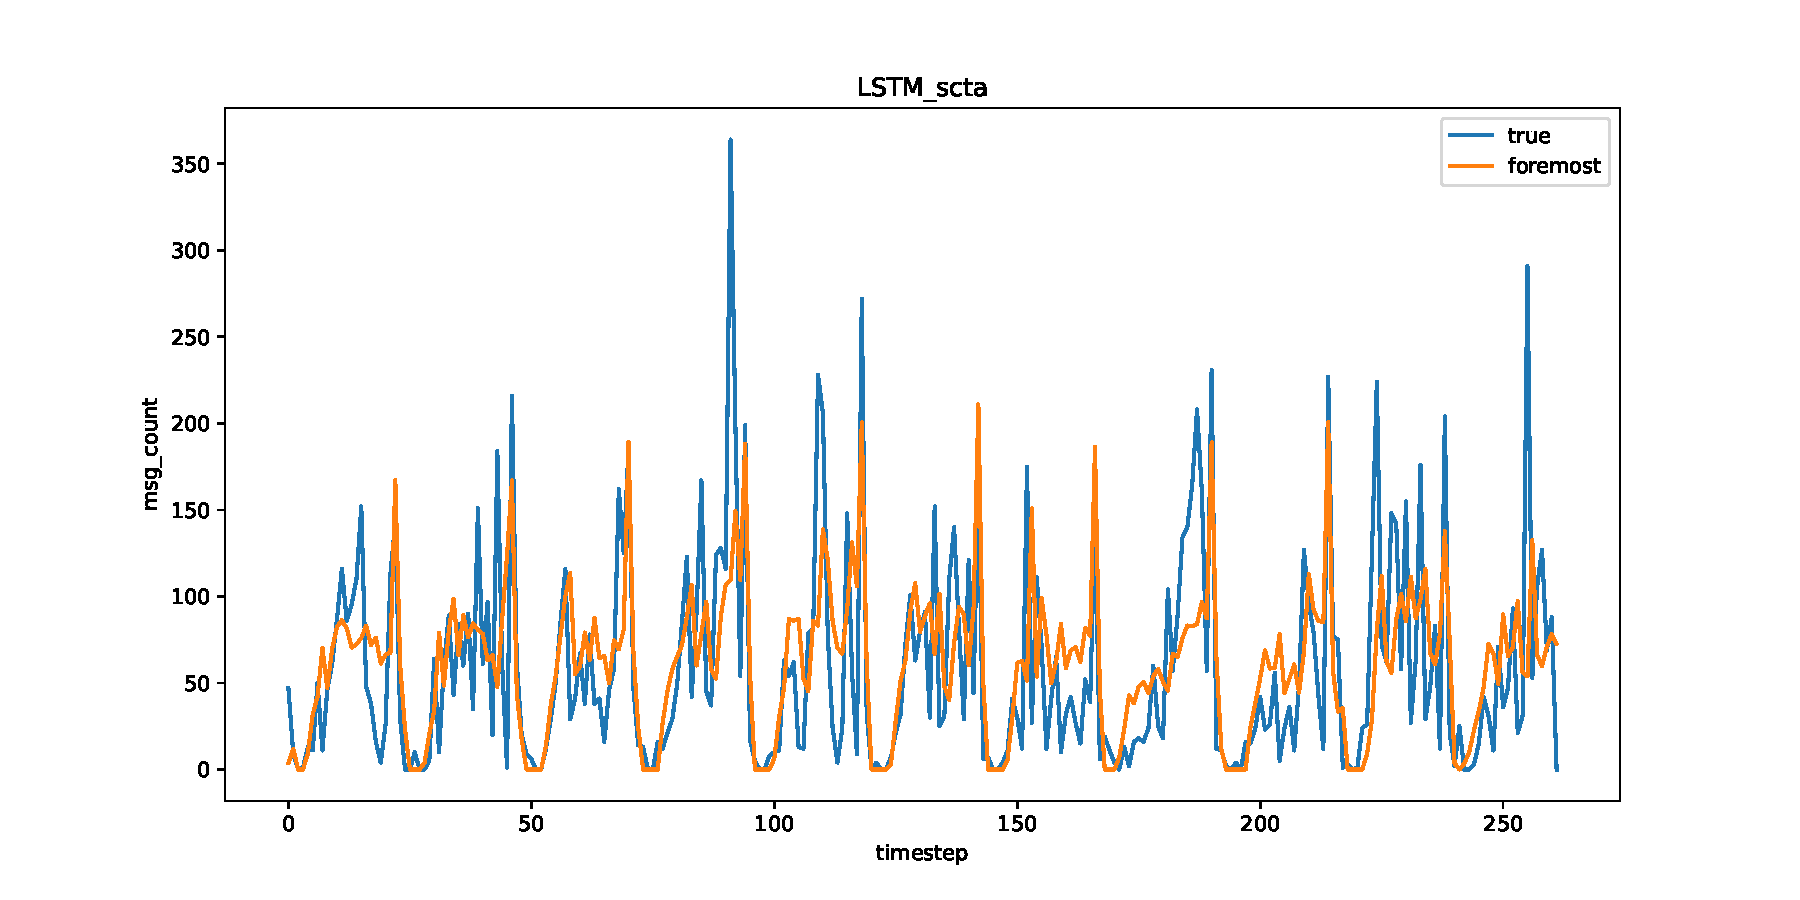
\includegraphics[width=0.8\textwidth]{/Users/justin/Desktop/data_analysis/graphs/LSTM_scta.pdf}
    \caption{LSTM 时间序列预测结果(scta)}
    \label{fig:lstm_scta}
\end{figure}

通过上述方法,LSTM 能够捕捉群聊消息数量随时间变化的趋势,并有效预测了未来时段的消息量。

\section{结论}
\subsection{研究结论}
\begin{itemize}
    \item \textbf{时间模式特征}:群聊活动展现出明显的日周期和工作日/周末差异。日内活跃高峰出现在晚间23:00至次日1:00,次高峰在10:00-12:00与17:00-19:00;工作日的群聊活跃度普遍高于周末。这一模式反映了高校学生群体的作息规律和社交习惯。

    \item \textbf{用户活跃度分布}:用户活跃度呈现显著的长尾分布特征。在772名用户中,仅19名超高活跃用户(约2.5\%)贡献了37.4\%的消息量,而55.3\%的低活跃用户仅贡献了总消息量的1.1\%。这种不均衡分布符合在线社群的普遍特征。

    \item \textbf{用户行为分类}:通过聚类分析成功识别出三类典型用户群体:高度活跃用户(平均7068.80条消息/人)、中度活跃用户(平均3402.57条消息/人)和低活跃用户(平均325.45条消息/人)。各群体在活跃时段和互动方式上均表现出独特特征。

    \item \textbf{内容特征}:文本消息(71.6\%)是主要交流方式,其次是图片(13.8\%)和表情(6.2\%)。高频词分析显示,除日常用语外,群聊内容紧密围绕东方Project相关话题展开,体现了明确的兴趣社群特征。
    
    \item \textbf{LSTM 预测}:通过LSTM模型对群聊消息数量进行时间序列预测,结果表明模型能够较好地捕捉消息数量的变化趋势。尽管存在一定的预测误差,但总体上模型对未来消息量的预测具有较高的准确性。帮助我们更好地理解和预测群聊活动的动态变化。
\end{itemize}

\subsection{讨论与展望}
\begin{itemize}
    \item \textbf{研究意义}:本研究通过大规模群聊数据分析,首次揭示了高校东方Project社群的在线互动模式,为理解年轻群体的社交行为提供了新的视角。

    \item \textbf{局限性}:当前研究仍存在数据收集时间跨度较短、样本群体范围有限等不足。同时,由于隐私保护考虑,未能深入分析用户间的社交网络结构特征。

    \item \textbf{未来方向}:建议后续研究可以:
        \begin{enumerate}
            \item 扩大数据收集范围,纳入更多群聊进行对比研究
            \item 结合社会网络分析方法,深入探究用户互动网络的形成和演化
            \item 引入自然语言处理技术,对群聊内容进行更深入的主题分析
            \item 探索建立预测模型,对群组活跃度和用户行为进行预测
        \end{enumerate}
\end{itemize}

\section*{附录}

本项目的所有代码已开源,同这份报告的 PDF 版本托管在 GitHub 上。代码包含数据预处理、LSTM 模型搭建与训练、性能评估以及可视化等完整实现。读者可以通过以下链接访问项目的详细内容:

\begin{itemize}
    \item GitHub 项目地址:\url{https://github.com/F1Justin/Quant-Group-Chat-Analysis}
    \item 代码仓库二维码:\\
\end{itemize}

\begin{center}
    
\includegraphics[width=0.3\textwidth]{/Users/justin/Desktop/data_analysis/graphs/qr-code.png} 
\end{center}

访问 GitHub 仓库以获取完整代码实现和详细说明。

\end{document}